
\subsection{Généralités}

La \english{partial reconfiguration} est un concept qui existait déjà dans les années 70 mais qui a vu le jour en 2009 lorsque les fabricants de puces \fpgas ont pris conscience des possibilités immenses de cette technologie. C'est l'arrivée des \fpgas{} qui a permis d'aboutir au développement de la \english{partial reconfiguration}.\\
Elle consiste à appliquer le procédé de reconfiguration sur une petite partie du \fpga{} en laissant fonctionner normalement la partie qui n'est pas reconfigurée. On parle aussi de reconfiguration à chaud, c'est-à-dire que le système n'est pas entièrement éteint lorsque l'opération est exécutée. Cela permet alors dans le cas d'un \english{System-On-Chip} de rajouter dynamiquement des modules sans devoir redémarrer le système. On peut alors concevoir un grand nombres de modules spécifiquement optimisés pour certaines applications (cryptologie, calcul flottants) pour lequel l'architecture initiale du processeur est peu optimale. Grâce au PR, la taille du \fpga{} n'est plus limitante puisque l'on peut implanter n'importe quel module. Cela permet de multiplexer temporellement les ressources du \fpga{} et d'économiser de l'énergie en enlevant des modules non utilisés.

\subsection{Les différents types de \english{partial reconfiguration}}

Il existe deux grands types de reconfigurations pour les \fpgas{} de \brand{Xilinx}. Il existe deux méthodes : \english{difference-based} et \english{module-based}.\\

La reconfiguration \english{difference-based} existait avant la \english{module-based}. La deuxième est un cas particulier de la première. La reconfiguration \english{difference-based} consiste à générer ce qu'on appelle un \english{partial bitstream} qui ne représentera que la différence d'une configuration initiale avec cette nouvelle configuration. Cette méthode est illustrée à la figure~\ref{partial-bitstream}. À partir de la configuration initiale et de ce \english{partial bitstream}, on obtient la deuxième configuration. Une option dans les outils de synthèse \brand{Xilinx} permet de générer un \english{bitstream} qui est la différence entre le premier système et le second. Le \fpga{} ne reconfigurera que les parties différentes.\\
\begin{figure}[h!]
\centering
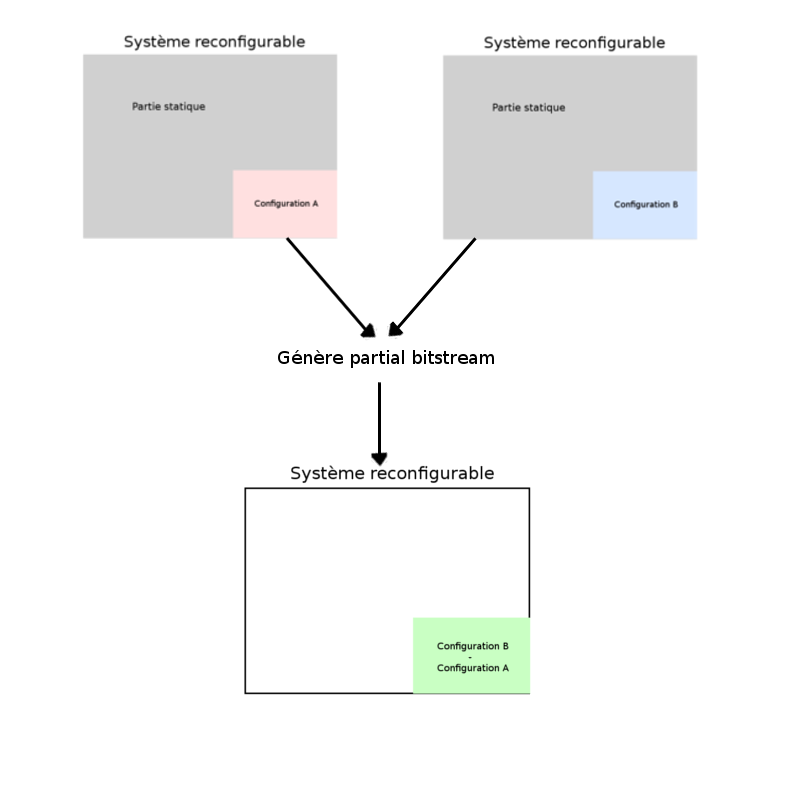
\includegraphics[scale=0.4]{pr2.png}
\caption{Génération d'un \english{partial bitstream}}
\label{partial-bitstream}
\end{figure}
Cette solution est adaptée pour des reconfigurations de petite envergure, mais assez peu efficace pour une solution plus complexe telle qu'envisagée dans le projet. En effet, la taille du \english{bitstream} grossit en fonction de la différence entre les deux circuits. Le but de notre projet est de pouvoir configurer à chaud un module appartenant à une \english{library} à développer.\\

La deuxième technique est la \english{partial reconfiguration module-based} qui consiste à segmenter le \fpga{} en zones. Il est ensuite possible d'instancier un module Verilog dans une zone. On appelle ces zones des tranches (\english{slices} en anglais). Il peut y avoir plusieurs tranches dans un projet mais il n'est possible d'allouer qu'un module par tranche à la fois. La reconfiguration s'effectue sur les tranches. Lors d'une reconfiguration, on assigne un module à une tranche, on dit qu'on l'instancie.\\
Considérons une carte mère qui contient des emplacements libres. Un qui peut contenir différents processeurs, un autre différentes cartes graphiques et un dernier qui peut contenir différentes cartes son. Ces emplacements représentent les tranches. Chaque composant représente un module qui peut être instancié dans son emplacement prévu.\\
Finalement, une configuration est une combinaison d'instances, chacune se trouvant dans une tranche. Une configuration est donc un triplet (processeur, carte graphique, carte son). Si le projet comporte trois tranches et trois modules instanciables par tranche alors le nombre de configurations possibles sera de $3^3=27$. Un module peut être instancié dans une tranche et pas dans une autre.\\
Le design doit au moins comporter une tranche dite statique, qui elle, ne peut être reconfigurée. La connexion entre les tranches statiques et les tranches reconfigurables est définie par des pins qui se situent à leurs frontières. Au moment de la conception, on choisit pour chaque tranche le nombre de \english{pins} qu'elle possède et leurs directions (ils ne peuvent être bidirectionel). Les \english{pins} reprèsentent la liaison entre la partie statique et la reconfigurable.\\

Cette méthode n'est pas compatible avec tous les \fpgas{} puisqu'il faut optimiser le routage entre les tranches et cette opération dépend de la plateforme utilisée. ISE, l'outil de gestion de projet et de synthèse de \brand{Xilinx}, ne le supporte pas pour la Spartan6.\\
Le projet étant complexe, la solution du \english{difference-based} ne convient pas.

\subsection{PlanAhead et l'incompatibilité avec la Spartan6}

Le logiciel PlanAhead de \brand{Xilinx} permet de définir les contraintes de routage et de placement des portes logiques d'un module afin qu'il puisse s'adapter à une tranche. Ces tranches sont aussi définies avec ce même logiciel, qui permet ensuite de générer les \english{bitstreams} correspondant à une configuration donnée. Malheureusement, PlanAhead ne permet pas de faire de \english{partial reconfiguration} sur Spartan6. En revanche, il permet de le faire uniquement sur les \fpgas{} suivants : Virtex-4, Virtex-5, Virtex-6, Virtex-7, Kintex-7, Artix-7 et Zynq.\\

Ayant fait une telle découverte, nous avons espéré utiliser la méthode \english{difference-based} pour simuler la méthode \english{module-based} en définissant clairement où se situent les différentes parties statiques et dynamiques. La partie statique étant fixée, il est possible en faisant la différence de deux configurations de faire disparaitre cette partie du \english{partial bitstream} puisqu'elle s'annule. L'inconvénient est qu'il faut alors générer un bitstream pour chaque configuration. Une pour passer d'une configuration $C_{1}$ à $C_{2}$, une de $C_{2}$ à $C_{3}$, une de $C_{1}$ à $C_{3}$ et leurs inverses. L'idée était alors de définir une configuration initiale appelée \english{blank} à partir de laquelle il est possible de se rendre dans n'importe quelle configuration et ensuite d'y revenir. Ainsi il est possible de réduire à deux le nombre de \english{partial bitstreams} à générer. Le fichier pour se rendre de Blank à $C_{x}$ et un fichier de $C_{x}$ à Blank.
